\documentclass[11pt]{article}
\usepackage{etex}
\usepackage[paper=letterpaper,margin=1in]{geometry}
\usepackage{graphics}
\usepackage{epsfig}
\usepackage{arcs}
\usepackage{fontenc}
\usepackage{alltt}
\usepackage{amssymb,amsfonts,epsf,url}
\usepackage{graphicx}
\usepackage{pstricks,pstricks-add}
\usepackage{pst-node}
\usepackage{pst-coil}
\usepackage{amsmath}
\usepackage{amsthm}
\usepackage{verbatim}

\usepackage{enumerate}
\usepackage{tikz}
\usepackage{amssymb,amsfonts}
\usepackage{amsmath,comment}


\usepackage{fancyhdr}

\newcommand{\pe}{\psi}
\newtheorem{theorem}{Theorem}[section]
\newtheorem{lemma}[theorem]{Lemma}
\newtheorem{corollary}[theorem]{Corollary}
\newtheorem{proposition}[theorem]{Proposition}
\newtheorem{observation}{Observation}
\newtheorem{case}[theorem]{Case}
\newtheorem{subcase}[theorem]{SubCase}
\newtheorem{transrule}[theorem]{TransRule}
\newtheorem{branchrule}[theorem]{BranchRule}
\newtheorem{remark}[theorem]{Remark}
\newtheorem{assumption}[theorem]{Assumption}
\newtheorem{definition}[theorem]{Definition}
\newtheorem{fact}[theorem]{Fact}
\newtheorem{reduction}{Reduction Rules}[section]
\renewcommand{\labelenumi}{\arabic{enumi}.}
\renewcommand{\labelenumii}{\arabic{enumi}.\arabic{enumii}.}
\renewcommand{\labelenumiii}{\arabic{enumi}.\arabic{enumii}.\arabic{enumiii}.}
\renewcommand{\labelenumiv}{\arabic{enumi}.\arabic{enumii}.\arabic{enumiii}.\arabic{enumiv}.}
\newlength{\alginputwidth}
\newlength{\algboxwidth}
\newcommand{\alginput}[1]{\makebox[1.5cm][l]{ {\sc Input:}} \parbox[t]{\alginputwidth}{{\it #1}}}
\newcommand{\algoutput}[1]{\makebox[1.5cm][l]{ {\sc Output:}} \parbox[t]{\alginputwidth}{{\it #1}}}
\newcommand{\algtitle}[1]{\underline{Algorithm \ {\bf #1}} \vspace*{1mm}\\}

\newsavebox{\algbox}
\newsavebox{\captionbox}
\newenvironment{algorthm}[2]{
        \setlength{\algboxwidth}{\columnwidth}
        \addtolength{\algboxwidth}{-\columnsep}
        \addtolength{\algboxwidth}{-1mm}
        \setlength{\alginputwidth}{\algboxwidth}
        \addtolength{\alginputwidth}{-1.7cm}
        \begin{figure}[tb]
            \vspace*{2mm}
            \centering
            \begin{lrbox}{\captionbox}
                \begin{minipage}[b]{\algboxwidth}
                    \centering
                    \caption{#1}
                    \label{#2}
                \end{minipage}
            \end{lrbox}
            \begin{lrbox}{\algbox}
                \begin{minipage}[b]{\algboxwidth}
                    \footnotesize
                    \vspace*{2mm}
    } {
                    \vspace*{0.2mm}
               \end{minipage}
            \end{lrbox}
            \fbox{\usebox{\algbox}\hspace*{1mm}}
            \usebox{\captionbox}
            \vspace*{-4mm}
        \end{figure}
    }
\newsavebox{\algcodebox}
\newenvironment{codeblock}{
        \begin{enumerate}
            \setlength{\itemsep}{2pt}
            \setlength{\parsep}{0pt}
            \setlength{\topsep}{0pt}
            \setlength{\parskip}{0pt}
            \setlength{\partopsep}{0pt}
    } {\end{enumerate}}
\newcommand{\step}{\item}
\newcommand{\paramproblem}[4]{\noindent {\sc #1}
\\
{\bf Given:} #2\\
{\bf Parameter:} #3\\
{\bf Question:} #4}


\newcommand{\YES}{\textup{\textsf{YES}}}
\newcommand{\NO}{\textup{\textsf{NO}}}
\newcommand{\Oh}{{\mathcal O}}
\newcommand{\Ohstar}{{\mathcal O^{*}}}
\newcommand{\nat}{\mathbb{N}}

\newcommand{\Pol}{\mbox{}}
\newcommand{\NP}{\mbox{}}
\newcommand{\APX}{\mbox{}}
\newcommand{\FPT}{\text{}}

\let\phi=\varphi
\let\epsilon=\varepsilon

\def\eg{{\em e.g.}}
\def\cf{{\em cf.}}
\def\ie{{\em i.e.}}
\def\etal{{\em et al.}}




\psset{unit=1pt}

\date{}
\title{On the Ordered List Subgraph Embedding Problems\footnote{A preliminary version of this paper appeared in proceedings of the {\em 8th International Symposium on Parameterized and Exact Computation} (IPEC), volume 8246 of {\em Lecture Notes in Computer Science}, pages~189--201, 2013.}}

\author{
{\sc Olawale Hassan}\footnote{School of
Computing, DePaul University, 243 S. Wabash Avenue, Chicago, IL
60604. Email: {\tt oahassan@gmail.com}, {\tt ikanj@cs.depaul.edu}, {\tt lperkovic@cs.depaul.edu}}
\and
{\sc Iyad Kanj}\footnotemark[2]
\and
{\sc Daniel Lokshtanov}\thanks{Department of Informatics,
University of Bergen, Bergen, Norway.  Email: {\tt daniello@ii.uib.no}}
\and
{\sc Ljubomir Perkovi\'{c}}\footnotemark[2]
}

\begin{document}

\maketitle

\begin{abstract}
In the (parameterized) {\sc Ordered List Subgraph Embedding} problem (p-OLSE) we are given two graphs  and , each with a linear order defined on its vertices, a function  that associates with every vertex in  a list of vertices in , and a parameter . The question is to decide if we can embed (one-to-one) a subgraph  of  of  vertices into  such that: (1) every vertex of  is mapped to a vertex from its associated list, (2) the linear orders inherited by  and its image under the embedding are respected, and (3) if there is an edge between two vertices in  then there is an edge between their images. If we require the subgraph  to be embedded as an induced subgraph, we obtain the {\sc Ordered List Induced Subgraph Embedding} problem (p-OLISE). The p-OLSE and p-OLISE problems model various problems in Bioinformatics related to structural comparison/alignment of proteins.

We investigate the complexity of p-OLSE and p-OLISE with respect to the following structural parameters: the {\em width}  of the function  (size of the largest list), and the maximum degree  of  and  of . In terms of the structural parameters under consideration, we draw a complete complexity landscape of p-OLSE and p-OLISE (and their optimization versions) with respect to the computational frameworks of classical complexity, parameterized complexity, and approximation.
\end{abstract}

\pagenumbering{roman}
\pagenumbering{arabic}

\section{Introduction} \label{sec:intro}
\subsection{Problem Definition and Motivation}
\label{subsec:motivation}
We consider the following problem that we refer to as the parameterized {\sc Ordered List Subgraph Embedding} problem, shortly (p-OLSE):

\paramproblem{} {Two graphs  and  with linear orders  and  defined on the vertices of  and ; a function ; and }{}{Is there a subgraph  of  of  vertices and an injective map  such that: (1)  for every ; (2) for every , if  then ; and (3) for every , if  then } \\

The parameterized {\sc Ordered List Induced Subgraph Embedding} (p-{\sc OLISE}) problem, in which we require the subgraph  to be embedded as an induced subgraph, is defined as follows:

\paramproblem{} {Two graphs  and  with linear orders  and  defined on the vertices of  and ; a function ; and }{}{Is there a subgraph  of  of  vertices and an injective map  such that: (1)  for every ; (2) for every , if  then ; and (3) for every ,  if and only if } \\

The optimization version of p-OLSE (resp. p-OLISE), denoted opt-OLSE (resp. opt-OLISE), asks for a subgraph  of  with the maximum number of vertices such that there exists a valid list embedding  that embeds  as a subgraph (resp. induced subgraph) into .

The p-OLSE and p-OLISE problems, and their optimization versions opt-OLSE and opt-OLISE, have applications in the area of Bioinformatics because they model numerous protein and DNA structural comparison problems (see~\cite{xiuzhen,evansphd,evans,xiuzhencai}).

In this paper we investigate the complexity of p-OLSE and p-OLISE with respect to the following structural parameters: the {\em width}  of the function  defined to be  and the maximum degree  of  and  of . Restrictions on the structural parameters ,  and  are very natural in Bioinformatics. The parameters  and  model the maximum number of hydrophobic bonds that an amino acid in each protein can have; on the other hand,  is usually a parameter set by the Bioinformatics practitioners when computing the top few alignments of two proteins~\cite{xiuzhencai}.

\subsection{Previous Related Results}\label{subsec:previous}
Goldman et al.~\cite{Goldman1999} studied protein comparison problems using the notion of {\em contact maps}, which are undirected graphs whose vertices are linearly ordered. They formulated the protein comparison problem as a {\sc Contact Map Overlap} problem, in which we are given two contact maps and we need to identify a subset of vertices  in the first contact map, a subset of vertices  in the second with , and an order-preserving bijection , such that the number of edges in  that correspond to edges in  is maximized. In~\cite{Goldman1999}, the authors proved that the {\sc Contact Map Overlap} problem is MAXSNP-complete, even when both contact maps have maximum degree one. The authors develop approximation algorithms by restricting their attention to special cases of the {\sc Contact Map Overlap} problem. In particular, they focus on cases where at least one of the graphs is a self-avoiding walk on the two dimensional grid.  Such walks are formulated as a one-to-one mapping  such that  for .  Goldman et al.~\cite{Goldman1999} observed that the geometry of proteins exhibit this structure, making self-avoiding walks a natural restriction for comparing protein contact maps.  They create contact maps from walks by taking the set  as the set of vertices and including an edge for every pair  such that  and . While the problem remains \NP-complete even when comparing two contact maps that are self-avoiding walks, the authors give a polynomial-time -approximation algorithm when comparing two self-avoiding walks and a polynomial-time -approximation algorithm when comparing a self-avoiding walk and an arbitrary contact map. The main difference between the {\sc Contact Map Overlap} problem and the opt-OLSE and opt-OLISE problems under consideration is that in opt-OLSE and opt-OLISE the bijection  is restricted to mapping a vertex to one in its list, and the goal is to maximize the size of the subgraph, not the number of edges, that can be embedded.


The p-OLISE problem generalizes the well-studied problem {\sc Longest Arc-Preserving Common Subsequence} (LAPCS) (see~\cite{gramm,evansphd,evans,guo,guohuidam,guohui}).  In LAPCS, we are given two sequences  and  over a fixed alphabet, where each sequence has arcs/edges between its characters, and the problem is to compute a longest common subsequence of  and  that respects the arcs. The LAPCS problem was introduced by~\cite{evansphd,evans} where it was shown to be -complete (parameterized by the length of the common subsequence sought) in the case when the arcs are {\em crossing}. Several works studied the complexity and approximation of LAPCS with respect to various restrictions on the types of the arcs (\eg, {\em nested}, {\em crossing}, etc.)~\cite{gramm,evansphd,evans,guo,guohuidam,guohui}. The work in~\cite{gramm,guo} considered the problem in the case of nested arcs parameterized by the total number of characters that need to be deleted from  and  to obtain the arc-preserving common subsequence. They showed that the problem is  with respect to this parameterization, and they also showed it to be  when parameterized by the length of the common subsequence in the case when the alphabet consists of four characters. The p-OLISE problem generalizes LAPCS since no restriction is placed on the size of the alphabet, and a vertex can be mapped to any vertex from its list. Consequently, the ``positive" results obtained in this paper about p-OLISE and opt-OLISE apply directly to their corresponding versions of LAPCS; on the other hand, we are able to borrow the -hardness result from~\cite{evans} to conclude the -hardness results in Proposition~\ref{prop:whardness} and Proposition~\ref{prop:whardness2}.

A slight variation of p-OLSE was considered in~\cite{xiuzhen,xiuzhencai}, where the linear order imposed on  and  was replaced with a partial order (directed acyclic graphs); the problem was referred to as the {\sc Graph Embedding} problem in~\cite{xiuzhen} and as the {\sc Generalized Subgraph Isomorphism} problem in~\cite{xiuzhencai}. The aforementioned problems were mainly studied in~\cite{xiuzhen,xiuzhencai} assuming no bound on  and  and, not surprisingly, only hardness results were derived. In~\cite{xiuzhencai}, a parameterized algorithm with respect to the treewidth of  and the map width  combined was given. Most of the hardness results in~\cite{xiuzhen,xiuzhencai} were obtained by a direct reduction from the {\sc Independent Set} or {\sc Clique} problems. For example, it was shown in~\cite{xiuzhen} that the problem of embedding the whole graph  into  is \NP-hard, but is in  if . It was also shown that the problem of embedding a subgraph of  of size  into  is -complete even when , and cannot be approximated to a ratio  unless ; we borrow these two hardness results as they also work for p-OLSE and p-OLISE.

Fagnot et al.~\cite{Fagnot2008178} introduced {\textsc Exact--Matching}, a problem in which we are given two graphs,  and , a mapping  as in p-OLISE and p-OLSE, and constants  and  where max and max. However,  there is no ordering imposed on the vertices of  or .  The objective is to find an injective homomorphism from  to . The authors proved that {\textsc Exact--Matching} is \NP-Complete when  and , even if  and  are bipartite graphs.  Fertin et al. in~\cite{Fertin2005,Fertin2009} revisited the original problem, restricting their attention to graphs of bounded degree, and considered an optimization version, {\textsc Max--Matching}, where the objective is to embed as many edges from  into  as possible. While the authors found that for small values of  and  there are cases where {\textsc Exact--Matching} is in  and cases where {\textsc Max--Matching} has a constant ratio approximation, generally the problem remains difficult. Fertin et al.~\cite{Fertin2005,Fertin2009} also give an  algorithm for solving {\textsc Max--Matching} by adding an arbitrary ordering to  and  which indicates that ordering  and  might improve the tractability of graph embedding problems. These results contrast with our results in Section~\ref{sec:complexity} and Section~\ref{subsec:parameterized} that show that p-OLSE and p-OLISE become easy when the ordering constraint is removed.

Finally, one can draw some similarities between p-OLISE and the {\sc Subgraph Isomorphism} and {\sc Graph Embedding} problems. The main differences between p-OLISE and the aforementioned problems are: (1) in p-OLSE we have linear orders on  and  that need to be respected by the map sought, (2) we ask for an embedding of a subgraph of  rather than the whole graph , and (3) each vertex must be mapped to a vertex from its list. In particular, requirement (1) above precludes the application of well-known (logic) meta-theorems (see~\cite{grohebook}) to the restrictions of p-OLISE that are under consideration in this paper.

\subsection{Our Results and Techniques}\label{subsec:results}
We draw a complete complexity landscape of p-OLSE and p-OLISE with respect to the computational frameworks of classical complexity, parameterized complexity, and approximation, in terms of the structural parameters ,  and . Table~1 outlines the obtained results about p-OLSE and p-OLISE and their optimization versions. Even though our hardness results are for specific values of the parameters , , and , these results certainly hold true for restrictions of the problems to instances in which the corresponding parameters are upper bounded by (or equal to --- by adding dummy vertices) any constant larger than these specific values. Observe also that the results we obtain {\em completely and tightly} characterize the complexity (with respect to all frameworks under consideration) of the problems with respect to ,  and  (unbounded vs. bounded, and when applicable, for different specific values).

Section~\ref{sec:complexity} presents various classical complexity results. The \NP-hardness results are obtained by a reduction from the \textsc{-Multi-Colored Independent Set} problem. Section~\ref{subsec:approximation} presents various approximation results for the optimization versions of p-OLSE and p-OLISE. Section~\ref{subsec:parameterized} presents parameterized complexity results for various restrictions of p-OLSE and p-OLISE. The -hardness results are obtained by tweaking the -hardness results given in the literature~\cite{xiuzhen,evans}, or by simple known reductions from the {\sc Independent Set} problem. The  results in Theorem~\ref{thm:mainboundeddegree} for p-OLSE, when , , and , are derived using the random separation method~\cite{cai}. This method is applied after transforming the problem --- via reduction operations --- to the {\sc Independent Set} problem on a graph composed of (1) a permutation graph and (2) a set of additional edges between the permutation graph vertices such that the number of additional edges incident to any vertex is at most a constant; Lemma~\ref{lem:separation} then shows that the {\sc Independent Set} problem on such graphs is . On the other hand, the  results in Proposition~\ref{prop:randomsimple}, when ,  (resp.  and  for p-OLISE by symmetry) and , are also derived using the random separation method~\cite{cai}, but the argument is simpler. We also explore the contribution of the ordering constraint of p-OLSE and p-OLISE to the difficulty of the problems.

To cope with the -hardness of p-OLSE in certain cases, we consider a different parameterization of the problem in Section~\ref{sec:vcnumber}, namely the parameterization by the vertex cover number, and denote the associated problem by p-VC-OLSE. This parameterization is not interesting for p-OLISE since we prove that p-OLISE is \NP-complete in the case when ,  and  = 1, and hence the problem is {\em para-\NP-hard}~\cite{grohebook} with respect to this parameterization. Proposition~\ref{prop:whardnessvc} shows that p-VC-OLSE is -complete in the case when ,  and  is unbounded (note that if either  or  then p-OLSE is  when ). So we restrict our attention to the case when , and show in this case that the problem is  even when both  and  are unbounded; the method relies on a bounded search tree approach, combined with the dynamic programming algorithm described in Proposition~\ref{prop:noedges}.



\begin{table}[htbp] \label{table:map}
\begin{center} \scriptsize
\mbox{\renewcommand{\arraystretch}{1.1}
\begin{tabular}{p{2.65cm}p{1cm}p{1cm}p{1cm}l}
{\small\bf p-OLSE}   & {\bf } & {\bf } & {\bf } & {\bf Complexity} \\ \hline
Classical     &  & 0 &  &  \\
              &  &  &  & -complete \\ \hline
Approximation &  &  &  & -complete \\
              &  &  &  &  not approximable to   \\ \hline
Parameterized &  &  &  &   \\
              &  &  &  & -complete \\
              &  &  &  & -complete  \\
              &  &  &  &  \\
              &  &  &  &  (even in ) \\ \hline
\end{tabular}}

\vspace*{0.5cm}

\mbox{\renewcommand{\arraystretch}{1.1}
\begin{tabular}{p{2.65cm}p{1cm}p{1cm}p{1cm}l}
{\small\bf p-OLISE}   & {\bf } & {\bf } & {\bf } & {\bf Complexity} \\ \hline
Classical     &  &  &  &  \\
              &  &  &  & -complete \\
              &  &  &  & -complete \\ \hline
Approximation &  &  &  & -complete \\
              &  &  &  &  not approximable to    \\
              &  &  &  &  not approximable to  \\ \hline
Parameterized &  &  &  & -complete \\
              &  &  &  & -complete \\
              &  &  &  &    \\
              &  &  &  &    \\
              &  &  &  & -complete \\
\end{tabular}}

\caption{Classical, approximation, and parameterized complexity maps of p-OLSE and p-OLISE with respect to ,  and . The inapproximability results are under the assumption that . The symbol  stands for unbounded degree.}
\end{center} \vspace*{-0.5cm}
\end{table}

\subsection{Background and Terminologies}\label{sec:background}
\paragraph{Graphs.} For a graph  we denote by  and  the set of vertices and edges of , respectively; we write  for .  For a set of vertices , we denote by  the subgraph of  induced by the vertices in . For a subset of edges , we denote by  the graph . For a vertex ,  denotes the set of neighbors of  in . The {\em degree} of a vertex  in , denoted , is .  A vertex  is {\em isolated} in  if . The {\em degree} of , denoted , is . A {\em matching} in a graph is a set of edges  such that no two edges in  share an endpoint. An {\em independent set} of a graph  is a set of vertices  such that no two vertices in  are adjacent.  A {\em maximum independent set} in  is an independent set of maximum cardinality.  A {\em clique} is subset of vertices  such that for each pair of vertices .  A {\em vertex cover} of  is a set of vertices such that each edge in  is incident to at least one vertex in this set; we denote by  the cardinality of a minimum vertex cover of . Let  and  be two parallel lines in the plane. A {\em permutation graph}  is the intersection graph of a set of line segments such that one endpoint of each of those segments lies on  and the other endpoint lies on . For more information about graphs, we refer the reader to~\cite{west}.

\paragraph{Optimization Problems.} An {\it \NP optimization problem}  is a 4-tuple .  is the set of input instances, which is recognizable in polynomial time. For each instance ,  is the set of feasible solutions for , which is defined by a polynomial  and a polynomial-time computable predicate  ( and  depend only on ) as . The function  is the objective function mapping a pair  and  to a non-negative integer.  The function  is computable in polynomial time. The function  is the {\em goal} function, which is one of the two functions , and  is called a {\it maximization problem} if , or a {\it minimization problem} if . We will denote by  the value , and if there is no confusion about the underlying problem , we will write  to denote .

\paragraph{Polynomial Time Approximation Algorithms.} A polynomial time algorithm  is an {\it approximation algorithm} for a (maximization)
problem  if for each input instance  the algorithm 
returns a feasible solution .  The solution 
has an {\it approximation ratio } if it satisfies the following
condition:


The approximation algorithm  has an {\it approximation ratio } if
for every instance  in  the solution  constructed by the
algorithm  has an approximation ratio bounded by .

An optimization problem  has a {\em constant-ratio approximation algorithm} if it has an approximation algorithm whose ratio is a constant.

Given two maximization problems  and , we say that  {\em L-reduces} to ~\cite{py91} if there are two polynomial-time computable functions/algorithms  and constants  and  such that:

\begin{enumerate}[(i)]
  \item For all ,  produces an instance  of , such that , and
  \item for any solution ,  produces a solution  such that~.
\end{enumerate}

\paragraph{Parameterized Complexity.} A {\it parameterized problem} is a set of instances of the form , where  for a finite alphabet set , and
 is a non-negative integer called the {\em parameter}.
A parameterized problem  is {\it fixed parameter tractable} (), if there exists an algorithm that on input 
decides if  is a yes-instance of  in time ,
where  is a computable function independent of ; we will denote by {\em fpt-time} a running time of the form .
A hierarchy of fixed-parameter intractability, {\it the -hierarchy} , was introduced based on the notion of {\em fpt-reduction}, in which the -th level  is the class .  It is commonly believed that . The asymptotic notation  suppresses a polynomial factor in the input length. For more information about parameterized complexity, we refer the reader to~\cite{fptbook,grohebook,rolfbook}.

\paragraph{Randomized Algorithms.} A {\em randomized algorithm} is an algorithm that relies on random data as part of its input.  Such algorithms can be {\em de-randomized} using techniques to enumerate values of the randomized input, yielding a deterministic algorithm.  In this paper we design randomized algorithms using the color coding technique introduced by Alon et al.~\cite{alon95} and the random separation technique introduced by Cai et al.~\cite{cai}.  Both techniques are applicable to problems where the objective is to find a subset of size  satisfying certain properties in a universe of size .

Given a problem where we seek a subset of size  satisfying certain properties in a universe of  elements, color coding works by randomly assigning  colors to the set of  elements and then looking for a subset of size  that is {\em colorful}, that is, where each element of the subset has a distinct color.  The algorithm can be de-randomized using families of -perfect hash functions, or colorings, constructed as shown in~\cite{alon95} in time . Thus, color coding algorithms run in time  where  is the running time to verify that a colorful subset of size  satisfying the desired properties exists for a given coloring.  If  is polynomial in , then the de-randomized algorithm runs in fpt-time.

Random separation~\cite{cai} works by randomly partitioning the vertices of a graph  into red and green vertices and testing whether a solution  exists such that  is entirely contained in the green partition and  is entirely contained in the red partition.  The likelihood that a solution  is colored green and  is colored red is .  To derandomize the algorithm we use -universal sets where .  Naor et al.~\cite{naor} give a construction of -universal sets that runs in time .  Thus, the running time for the de-randomized algorithm is , where  is the time it takes to verify that a solution exists in the green partition and its neighbors are in the red partition.  If  is polynomial in  and  is bounded by a function of  then the algorithm runs in fpt-time.

We will denote an instance of p-OLSE or p-OLISE by the tuple . We shall call an injective map  satisfying conditions (1)-(3) in the definition of p-OLSE and p-OLISE (given in Section~\ref{sec:intro}) for some subgraph  of , a {\em valid list embedding}, or simply a {\em valid embedding}. Constraint (3) will be referred to as the {\em embedding constraint} (note that constraint (3) is different in the two problems). We define the {\em width} of , denoted , as . It is often more convenient to view/represent the map  as a set of edges joining every vertex  to the vertices of  that are in .

\section{Classical Complexity Results}\label{sec:complexity}
In this section we consider p-OLSE and p-OLISE, and their optimization versions, with respect to classical complexity. Consider the restrictions of the opt-OLSE and opt-OLISE problems to instances in which  (for p-OLSE we can even assume that  as the edges in  do not play any role when ). This version of the problem can be easily shown to be solvable in polynomial time by dynamic programming. The algorithm is very similar to that of the {\sc Longest Common Subsequence} problem; so we only give the recursive definition of the solution necessary for the dynamic programming approach.

\begin{proposition}\label{prop:noedges}
The opt-OLSE problem restricted to instances in which  and  , and the opt-OLISE problem restricted to instances in which  are solvable in  time (and hence are in ).
\end{proposition}

\begin{proof}
Assume that the vertices of  are ordered as  with respect to , and that the vertices of  are ordered as  with respect to .
We maintain a two-dimensional table , in which  is the maximum cardinality of a subset of  from which there exists a valid list embedding into . The entry  can be computed recursively as follows:  if , and  otherwise. We can now use a standard dynamic programming approach to compute  and to construct the subgraph  and the embedding . The running time of the algorithm is .
\end{proof}

Proposition~\ref{prop:noedges} will be useful for Proposition~\ref{prop:apx} and Theorem~\ref{thm:fptvslose}.

As we show next, if , the p-OLSE and p-OLISE problems become -complete, even in the simplest case when ,  and . The same proof shows the \NP-completeness
of p-OLISE when ,  and  by symmetry.


\begin{theorem}
The p-OLSE and p-OLISE problems restricted to instances in which , , and  are -complete.
\end{theorem}

\begin{proof}
We first present the proof for p-OLSE.

It is easy to see that p-\textsc{OLSE} , so it suffices to show that
p-\textsc{OLSE} is -hard.  We do so by providing a polynomial time
reduction from the \textsc{-Multi-Colored Independent Set (-MCIS)} problem:
decide whether for a given graph  and a proper -coloring of the
vertices , where  and each color class has the same cardinality, there exists an independent
set  of size  such that, , ~\cite{Hartung2013}.

Let  be an instance of \textsc{-MCIS}.
We assume that the set , , of vertices that are mapped to color 
is of size , and we label the vertices of   such that
 (see Figure~1). We
describe how we construct the corresponding instance  of p-\textsc{OLSE}.

\begin{figure}
\label{fi:kMCIS}
\begin{center}
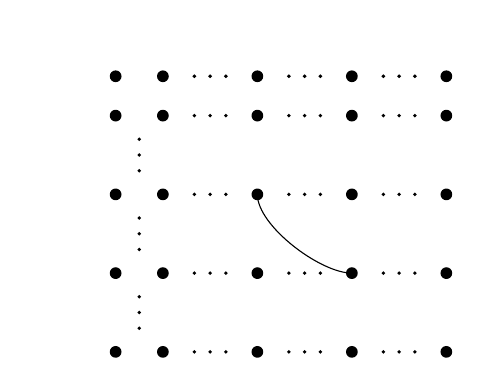
\begin{tikzpicture}
[vertex/.style={fill,circle,inner sep = 1.5pt},
dot/.style={fill,circle,inner sep = 0.5pt}]

\node at (0,4) [color=gray] {\tiny};
\node at (0.6,4) [color=gray] {\tiny};
\node at (1.8,4) [color=gray] {\tiny};
\node at (3,4) [color=gray] {\tiny};
\node at (4.2,4) [color=gray] {\tiny};

\foreach \y in {0,1,2,3,3.5}
{
  \foreach \x in {0,0.6,1.8, 3,4.2}
  {
    \node at (\x, \y) [vertex] {};
  }
  \draw (1,\y) node[dot] {};
  \draw (1.2,\y) node[dot] {};
  \draw (1.4,\y) node[dot] {};
  \draw (2.2,\y) node[dot] {};
  \draw (2.4,\y) node[dot] {};
  \draw (2.6,\y) node[dot] {};
  \draw (3.4,\y) node[dot] {};
  \draw (3.6,\y) node[dot] {};
  \draw (3.8,\y) node[dot] {};
}
\node at (-1,3.5) {};
\node at (-1,3) {};
  \draw (0.3,2.7) node[dot] {};
  \draw (0.3,2.5) node[dot] {};
  \draw (0.3,2.3) node[dot] {};
\node at (-1,2) {};
  \draw (0.3,1.7) node[dot] {};
  \draw (0.3,1.5) node[dot] {};
  \draw (0.3,1.3) node[dot] {};
\node at (-1,1) {};
  \draw (0.3,.7) node[dot] {};
  \draw (0.3,.5) node[dot] {};
  \draw (0.3,.3) node[dot] {};
\node at (-1,0) {};

\draw (1.8,2) node[label=90:{}] {};
\draw (3,1) node[label=90:{}] {};
\draw (1.8,2) .. controls +(-90:0.4cm) and +(180:0.4cm) .. (3,1);
\end{tikzpicture}
\end{center}
\caption{An instance of \textsc{-MCIS} consists of  vertices partitioned
into  color classes  each of size . All edges are
between vertices in different color classes. The edge , for
example, connects vertices  and  where  and
.}
\end{figure}

To construct , we associate with every color class  a
block  of vertex sequences  such that each , ,
is a sequence of  vertices .  is then
the set of all vertices  for , , and
. The ordering  of vertices in  is defined as
follows: for all 

(See Figure~2-(a).) Lastly we define the set  as follows: 
is an edge in  if and only if , , ,
and . (See Figure~2-(b).)

\begin{figure}
\label{fig100}
\begin{tikzpicture}
[vertex/.style={fill,circle,inner sep = 1.5pt},
dot/.style={fill,circle,inner sep = 0.5pt}]



\node at (-2, 0) {a)};
\node at (-1, 0) {};

\foreach \x in {0,3.5,8}
{
  \draw [color=gray] (\x-0.5,-0.3) rectangle (\x+2.1,0.9);
  \foreach \e in {0, 0.5, 1.5}
  {
    \node at (\x+\e, 0) [vertex] {};
  }
  \draw (\x+0.8,0) node[dot] {};
  \draw (\x+1,0) node[dot] {};
  \draw (\x+1.2,0) node[dot] {};
}

\draw (6.25,0) node[dot] {};
\draw (6.5,0) node[dot] {};
\draw (6.75,0) node[dot] {};

\node at (0,0) [label=90:{}] {};
\node at (1.5,0) [label=90:{}] {};

\node at (3.5,0) [label=90:{}] {};
\node at (5,0) [label=90:{}] {};

\node at (8,0) [label=90:{}] {};
\node at (9.5,0) [label=90:{}] {};

\node at (0.75,-0.8) {};
\node at (4.25,-0.8) {};
\node at (8.75,-0.8) {};
\end{tikzpicture}

\vspace{0.7cm}
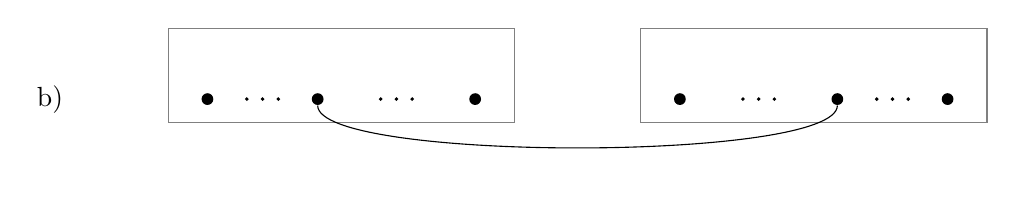
\begin{tikzpicture}
[node/.style={fill,circle,inner sep = 1.5pt},
dot/.style={fill,circle,inner sep = 0.5pt}]


\node at (-4,2) {b)};

\draw (-2,2) node[node,label=90:{}] {};
\draw (-1.5,2) node[dot] {};
\draw (-1.3,2) node[dot] {};
\draw (-1.1,2) node[dot] {};
\draw (-0.6,2) node[node,label=90:{}] (u) {};
\draw (0.2,2) node[dot] {};
\draw (0.4,2) node[dot] {};
\draw (0.6,2) node[dot] {};
\draw (1.4,2) node[node,label=90:{}] {};

\draw [color=gray] (-2.5,1.7) rectangle (1.9,2.9) {};
\node at (-1.2,1.2) {};

\draw (4,2) node[node,label=90:{}] {};
\draw (4.8,2) node[dot] {};
\draw (5,2) node[dot] {};
\draw (5.2,2) node[dot] {};
\draw (6,2) node[node,label=90:{}] (up) {};
\draw (6.5,2) node[dot] {};
\draw (6.7,2) node[dot] {};
\draw (6.9,2) node[dot] {};
\draw (7.4,2) node[node,label=90:{}] {};

\draw [color=gray] (3.5,1.7) rectangle (7.9,2.9) {};
\node at (6.8,1.2) {};

\draw (u) .. controls +(-90:0.8cm) and +(-90:0.8cm) .. (up);

\end{tikzpicture}
\caption{a) Associated with every color class  is a block  of vertex
sequences  such that each  is a sequence of 
vertices . The vertex sequences 
correspond to the  vertices of . b) 
is an edge in  if and only if , ,
and .}
\end{figure}


To construct , we again associate with every color class
 a block  of vertex sequences  such that each
 is a sequence of  vertices .
 is the set of all vertices  for ,
, and . The ordering  of vertices
in  is defined just as it was in .
The edge set  is simply : in this way, for any valid list embedding
, where  is a subgraph of ,  must be an independent
set of .

We complete the construction of the instance of p-\textsc{OLSE} by defining
the mapping .  is a bijection that maps the vertices in each block
 to the block  as follows:

This mapping is illustrated in Figure~3.

\begin{figure}
\label{fi:map}
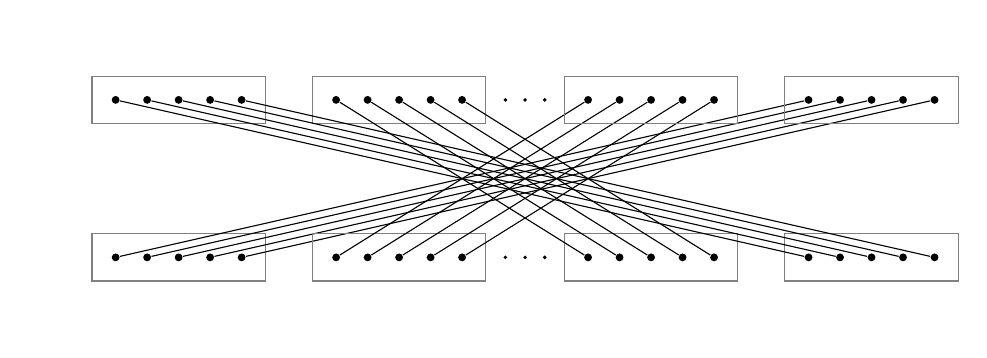
\begin{tikzpicture}
[vertex/.style={fill,circle,inner sep = 1pt},
dot/.style={fill,circle,inner sep = 0.5pt}]

\node at (-1, 0) {};
\node at (-1, 2) {};

\foreach \x in {0,2.8, 6,8.8}
{
  \draw [color=gray] (\x-0.3,-0.3) rectangle (\x+1.9,0.3);
  \draw [color=gray] (\x-0.3,1.7) rectangle (\x+1.9,2.3);
  \foreach \e in {0, 0.4, 0.8, 1.2, 1.6}
  {
    \node at (\x+\e, 0) [vertex] (h) {};
    \node at (8.8-\x+\e, 2) [vertex] (l) {};
    \draw (h) -- (l);
  }
}

\draw (4.95,2) node[dot] {};
\draw (5.2,2) node[dot] {};
\draw (5.45,2) node[dot] {};
\draw (4.95,0) node[dot] {};
\draw (5.2,0) node[dot] {};
\draw (5.45,0) node[dot] {};

\node at (0.8,-0.8) {};
\node at (0.8,2.8) {};

\node at (3.6,-0.8) {};
\node at (3.6,2.8) {};

\node at (6.8,-0.8) {};
\node at (6.8,2.8) {};

\node at (9.6,-0.8) {};
\node at (9.6,2.8) {};
\end{tikzpicture}
\caption{The mapping  maps vertices of  to vertices of . More
precisely, it maps vertices of  to vertices of  in a way
that forbids an embedding that would map a vertex in  and a vertex in
 simultaneously, for any , , .}
\end{figure}


This completes the construction of the instance of p-OLSE. Observe that in the constructed instance we have , , and . We show next that  has an independent set of size  if and only if the constructed instance of p-OLSE has a subgraph  of  of size , and a valid embedding
.

Let  be solution to the instance  of \textsc{-MCIS}. Each vertex  corresponds to a
sequence  where .
For any two sequences , there is an edge
between a vertex of  and a vertex of  if and only if
 for  and  (). Since for
every pair  and since
, there are  sequences  with the property
that for any two vertices  and
, .
By construction of , the vertices of any two sequences 
() that do not have edges between them are simultaneously embeddable in . Therefore,
we can define a valid embedding , where , and  consists of all the vertices in each 
that corresponds to a vertex in .

Conversely, let , , be a valid embedding
from a subgraph  of  into .  By construction of ,  can embed at most 
vertices from any block  into  and, furthermore, all vertices
in  embedded by  must belong to the same sequence  of
. Therefore, exactly  sequences, one from each of the  blocks, are fully embedded by . Moreover, because ,  embeds all  vertices of
the  sequences  in  if and only if for any two vertices
.
By construction of , each sequence  corresponds to the 
vertex of the color class . Therefore, we can find a subset
 such that for any two vertices  and ; that is, the set
 is a solution to the instance  of \textsc{-MCIS}.

 For p-OLISE, since , the same reduction given above can be used to show its -hardness when ,  and .  To show that p-OLISE is \NP-hard when ,  and  we need only tweak the construction of the p-OLISE instance as follows.  We construct  as we constructed  in the previous case (with edges), and we construct  as we constructed  in the previous case (without edges). The \NP-hardness when ,  and  follows by symmetry.
\end{proof}

We contrast this hardness result with a result for a version of the problem where the injective map need not preserve the ordering of the vertices.  First, we define the parameterized {\sc List Subgraph Embedding} problem (p-LSE):

\paramproblem{} {Two graphs  and ; a function ; and }{}{Is there a subgraph  of  of  vertices and an injective map  such that: (1)  for every  and (2) for every , if  then } \\

\begin{proposition}\label{prop:pLSE-in-P}
The p-LSE problem restricted to instances where , , and  is in .
\end{proposition}
\begin{proof}
It suffices to prove that the optimization version opt-LSE of p-LSE is in .

For each vertex  define . Note that for each ,  defines a subset of vertices in  from which only one vertex can be included in the solution.  Let  be the set of subsets of  where . Since , the elements of  are pairwise disjoint. We say that two subsets  and , , are {\em adjacent} if there exists an edge  where  and .  We define a {\em cycle} of subsets to be a sequence of distinct subsets , , such that  and  are adjacent, for , and  and  are adjacent; or a sequence of two subsets  such that there are two distinct vertices  in  and two distinct vertices  in  such that  is adjacent to  and  is adjacent to .  Using these constructs, we can define the following rules to simplify the problem:

\begin{enumerate}[(i)]
  \item For each subset  with a vertex  such that , or  has a neighbor in , we add  to the solution  and we define . We remove the vertices in  from  and vertex  from .

  \item For each cycle of subsets , if , choose two vertices  in each ,  such that  is adjacent to , for , and  is adjacent to . Add  to the solution , define , and remove the vertices in  from  and  from , for . If , let  and  such that  is adjacent to  and  is adjacent to . Add  to the solution , define , , and remove the vertices in  from  and  from .
\end{enumerate}

Clearly, each of the above rules is safe in the sense that it is possible to extend the solution obtained after each application of the rule to an optimal solution. After the above rules are no longer applicable, we are left with a graph  (we call the resulting graph  for simplicity) where the remaining subsets in  (considered as nodes), together with their adjacency relation, form a tree-like structure.  We say that a subset  is a {\em leaf-subset} (in ) if it is adjacent to exactly one other subset in ; observe that every subset  must be adjacent to at least one other subset in  by rule (i). Since each leaf-subset is adjacent to one subset in , each leaf-subset must consist of exactly one vertex for the following reasons. First, by rule (i), each vertex in a leaf-subset  must have a neighbor in the (single) subset  that is adjacent to . By rule (ii),  must consist of exactly one vertex; otherwise, rule (ii) would apply to  and . To complete the construction of our solution, we iteratively apply a new rule, rule (iii), that includes the vertex  in our solution , for each leaf-subset , defines , and removes the vertices in  from  and  from . Rule (iii) is safe because any optimal solution must contain exactly one of  and its only neighbor  in the subset adjacent to , and in the case when the solution contains ,  can be exchanged with , and the map  can be updated by defining . When rule (iii) is no longer applicable, the graph  is empty, and the algorithm has computed an optimal solution.  Clearly, the running time is polynomial because each application of a rule removes at least one vertex from  (and from ). \end{proof}

\section{Approximation Results}\label{subsec:approximation}
In this section we consider opt-OLSE and opt-OLISE with respect to the framework of approximation theory. We begin with the following proposition:

\begin{proposition}\label{prop:apx}
The opt-OLSE problem restricted to instances in which  has an approximation algorithm of ratio , and the opt-OLISE problem restricted to instances in which  and  has an approximation algorithm of ratio .
\end{proposition}

\begin{proof}
Let  be an instance of opt-OLSE, and consider the following algorithm. Apply the dynamic programming algorithm in Proposition~\ref{prop:noedges} to  after removing the edges of  and the edges of , and let  and  be the subgraph and map obtained, respectively. Apply the following trivial approximation algorithm to compute an independent set  of : pick a vertex  in , include  in , remove  and  from , and repeat until  is empty.  Return the subgraph , and the restriction of  to , . Clearly, we have .

Since  is a valid list embedding of  after the edges of  and  have been removed, and since  is an independent set of , it is clear that  is a valid list embedding of  into . Therefore, the algorithm is an approximation algorithm. Now let  be an optimal solution of the instance.  is an upper bound on the size of an optimal solution  since  is a solution to opt-OLSE that respects the embedding constraint. Therefore, .

For opt-OLISE, we apply the algorithm above to obtain , however, there may be vertices  where , violating the embedding constraint of opt-OLISE.  We use a similar method to that used to obtain the approximation algorithm described above to overcome this hurdle. This time we pick a vertex  in the image  of the independent set , include  in the independent set , remove  and  from , and repeat until  is empty. As was the case for , it follows that . Let  be the inverse image . Since  and , it follows that .  remains an upper bound on the size of an optimal solution . Therefore, . \end{proof}

The inapproximability results outlined in Table~1 follow by simple reductions from the {\sc Maximum Independent Set} problem.  We introduce the following reduction modeled after a reduction in \cite{xiuzhen} for a variation of opt-OLSE.

\begin{lemma}
\label{lem:reduce-IS}
Let  be a graph.  Construct an instance  of opt-OLSE from  as follows. Let  be an arbitrary ordering on the vertices of ,  where .  Let  be the graph consisting of the isolated vertices , where .  Define the mapping  such that for each vertex , . We have:
\begin{enumerate}[(i)]
  \item  has an independent set of size  if and only if  has a solution of size .
  \item There is an fpt-reduction from \textsc{Independent Set} to p-OLSE where  and , and to p-OLISE where ,  (resp. ,  by symmetry) and .
  \item There is an L-reduction from \textsc{Maximum Independent Set} to opt-OLSE where  and , and to opt-OLISE where ,  (resp. ,  by symmetry) and .
\end{enumerate}
\end{lemma}

\begin{proof}

(i) Let  be an independent set in  where .  Since , for any subgraph  of  and a valid embedding , no two vertices  are adjacent. Given that  is an independent set and that for each vertex , letting , we can define the embedding , where  for , satisfying that for any two vertices  if  then .  Thus, there is a valid embedding from  to  where .

Conversely, let  be an embedding where  is a subgraph of  satisfying .  As observed earlier,  must be an independent set since . Thus,  has an independent set  where .

(ii) Let  be an instance of \textsc{Independent Set}. We construct the instance \newline  by following the same procedure outlined in the statement of the lemma.  By part (i),  contains an independent set  where  if and only if there exists a valid embedding  where . Since the same parameter is shared between the instance of \textsc{Independent Set} and the instance  of p-OLSE, and since the construction of  can be clearly done in polynomial time, we have an fpt-reduction from \textsc{Independent Set} to p-OLSE. The reduction extends immediately to the case of p-OLISE where ,   and  because .  By symmetry, it also can be used for the case of p-OLISE where ,  and .

(iii) The -reduction is given by the function  that maps the instance  of \textsc{Maximum Independent Set} into the instance  of opt-OLSE, as described in the statement of the lemma, and the function  that, for each solution  of  corresponds the solution  of , and the constants . By part (i), any solution  of  corresponds to a solution  of  such that , and vice versa. Therefore, , and . This shows that \textsc{Maximum Independent Set} -reduces to opt-OLSE.

The -reduction extends immediately to the case of opt-OLISE where  and , and by symmetry it extends to the case of opt-OLISE where  and . \end{proof}

We can now demonstrate that opt-OLSE is APX-complete when  and opt-OLISE is APX-complete when  and .

\begin{proposition}\label{prop:apx-complete}
The opt-OLSE problem restricted to instances in which  and the opt-OLISE problem restricted to instances in which  and  are APX-complete.
\end{proposition}

\begin{proof}
Proposition~\ref{prop:apx} showed that opt-OLSE is in APX when . We demonstrate that opt-OLSE is APX-complete when  and  to yield the result. Since the case of opt-OLSE where ,  and  is a subset of opt-OLSE where ,  and  we can apply Lemma~\ref{lem:reduce-IS} part (iii) to -reduce {\sc Maximum Independent Set} to the cases of opt-OLSE where  has bounded degree.  Since {\sc Maximum Independent Set} on bounded degree graphs is APX-complete, it follows that opt-OLSE is APX-complete when ~\cite{py91}.  Similar arguments can be applied to opt-OLISE to show that it is APX-complete when restricted to instances in which  and .
\end{proof}

The inapproximability results for opt-OLSE and opt-OLISE when ,  and  (and the symmetric case for opt-OLISE when  ,  and ) also follow from Lemma~\ref{lem:reduce-IS}.

\begin{proposition}\label{prop:no-apx}
The opt-OLSE problem restricted to instances in which  and  and opt-OLISE restricted to instances in which  and  or  and  cannot be approximated to within a factor of  unless , where  is the number of vertices in .
\end{proposition}

\begin{proof}
H\r{a}stad demonstrated in~\cite{hastad97} that {\sc Maximum Independent Set} is not approximable to within a factor of , for any , unless .  The proposition follows immediately from the -reduction in part (iii) of Lemma~\ref{lem:reduce-IS} for the given cases of opt-OLSE and opt-OLISE.
\end{proof}

\section{Parameterized Complexity Results}\label{subsec:parameterized}

In this section we consider p-OLSE and p-OLISE with respect to the framework of parameterized complexity. Applying part (ii) of Lemma~\ref{lem:reduce-IS} to p-OLSE and p-OLISE yields the following result:

\begin{proposition}
\label{prop:whardness1}
The p-OLSE problem restricted to instances in which ,  and  is -complete, and the p-OLISE problem restricted to instances in which ,  (resp.  and  by symmetry) and  is -complete.
\end{proposition}

\begin{proof}
Downey and Fellows showed in~\cite{df2} that \textsc{Independent Set} is -complete.  By part (ii) of Lemma~\ref{lem:reduce-IS} there is an fpt-reduction from \textsc{Independent Set} to p-OLSE restricted to instances in which ,  and , and to p-OLISE restricted to instances in which ,  (resp.  and  by symmetry) and . The statement of the proposition follows.
\end{proof}

Next, we consider the case of p-OLSE and p-OLISE when ,  and . Evans~\cite{evans} reduces the -complete problem {\sc Clique}~\cite{fptbook} to the {\sc Longest Arc-Preserving Common Subsequence} (LAPCS) to show that LAPCS is -hard when the length of the common subsequence, , is the parameter, and when no two arcs in the instance share an endpoint. The reduction encodes a graph  as an arc-annotated sequence  where each vertex in  is a substring of  of the form  and where the edges in  are encoded as arcs between the substrings of  with endpoints corresponding to the endpoints of the edge in .  A clique of size  is encoded as an arc-annotated sequence  where each of the  vertices in the clique is encoded as a substring of  of the form  with similarly constructed arcs between substrings.  A clique of size  exists in  if  is an arc-preserving subsequence of  with length .  Since the length of , is a function of , {\sc Clique} is fpt-reducible to LAPCS.

We show that LAPCS is a special case of p-OLISE where  and .  Taking each character in  and  to be a vertex in  and , respectively, and preserving the arcs in  and  as edges in  and , respectively,  and  are reduced to the graphs  and , respectively, and . Each vertex  has a list in  that consists of the vertices  such that the character for  is the same as the character for .  The size of the parameter  remains the same, completing the reduction of LAPCS to p-OLISE.  Note that a clique of size  is encoded by the property that the embedding from  to  preserves the arcs in , which is a property of solutions for both p-OLSE and p-OLISE.  Thus, by the same arguments, LAPCS reduces to p-OLSE as well.  Finally, note that this reduction results in instances of p-OLSE and p-OLISE where the question is whether we can embed the whole graph  into , yielding the following proposition:

\begin{proposition}\label{prop:whardness}
The p-OLSE and p-OLISE problems restricted to instances in which  and  are -complete.  Moreover, the problems remain -complete when the parameter  is the number of vertices in .
\end{proposition}

\begin{proposition}\label{prop:whardness2}
The p-OLISE problem restricted to instances where , , and  is -complete under Turing fpt-reductions.
\end{proposition}

\begin{proof}
Let  be the set of instances of p-OLISE where , , and .  For an instance  define  where, for each . As a consequence of , for every instance , and for every vertex , we have . Let  be the set of all .  It is easy to see that an instance of p-OLISE  is a yes-instance if and only if  is a yes-instance.  Therefore, to prove the proposition we can equivalently prove that p-OLISE restricted to instances in  is -complete.  Denote by p-OLISE-simple p-OLISE restricted to instances in which , , , and .  Proposition~\ref{prop:whardness} showed that p-OLISE-simple is -complete.  We give a Turing fpt-reduction from p-OLISE-simple to  to yield the result.

Let  be an instance of p-OLISE-simple where .   Using color-coding, there is a family  of fpt-many -colorings for the vertices in  using the colors  --- corresponding to the labels of the vertices of  --- such that if  is a yes-instance, then there is a coloring , and a valid embedding  , such that  if and only if .  To reduce , for every coloring  we create the instance  of p-OLISE where , where for each , .  Observe that by the definition of , for each vertex , .  Thus, .

Hence there is a Turing fpt-reduction from p-OLISE-simple to , and if there is an algorithm that runs in fpt-time that solves , then we can find a solution for p-OLISE-simple in fpt-time by enumerating the colorings in  and applying the algorithm for . Given that p-OLISE-simple is -complete, it follows that  is -complete under Turing fpt-reductions.  It follows that  is -complete as well under Turing fpt-reductions.
\end{proof}

Again, relaxing the ordering constraint significantly reduces the difficulty of the problem.  For example, when we relax the ordering constraint in p-OLISE we have the parameterized {\sc List Induced Subgraph Embedding} problem, shortly (p-LISE):

\paramproblem{} {Two graphs  and ; a function ; and }{}{Is there a subgraph  of  of  vertices and an injective map  such that: (1)  for every  and (2) for every ,  if and only if } \\


\begin{proposition}\label{prop:unordered_is_in_P}
The p-LISE problem restricted to instances in which  and  is in .
\end{proposition}

\begin{proof}
It suffices to show that the optimization (maximization) version opt-LISE of p-LISE is in . We proceed by reducing opt-LISE in the case where  and  to the well-known polynomial-time computable problem \textsc{Weighted Maximum Matching on Bipartite Graphs} (WMMBG):  Given a graph , a bipartition , and weight function , find a matching  with maximum weight, where the weight of a matching .

Let  be an instance of opt-LISE.  To create , we first create the vertices of  from the edges and vertices of .  For each edge  where , we add a vertex to .  For each vertex  where , we add a vertex to .  We follow the same procedure to create the vertices of  from .  To complete  we add edges as follows:

\begin{enumerate}[(i)]
 \item For any two edges  and  such that  and , we add an edge of weight 2 between the vertex in  corresponding to  and the vertex in  corresponding .
 \item For each vertex  such that  and for each vertex  such that , we add an edge of weight 1 between the vertex corresponding to  in  and the vertex corresponding to  in .

 \item For each vertex  such that , and for each vertex  with neighbor , we add an edge of weight 1 between the vertex corresponding to  in  and the vertex corresponding to the edge  in . If both  and  appear in  we add {\em only} one edge between the vertex corresponding to  in  and that corresponding to  in  so that no multi-edges are created in .

 \item Finally, for each vertex  with neighbor  in , and for each vertex  where , we add an edge of weight 1 between the vertex in  corresponding to  and the vertex in  corresponding to . If  appears in both  and , we add {\em only} one edge between the vertex corresponding to  in  and that corresponding to  in  so that no multi-edges are created in .
\end{enumerate}

This completes the construction of .  We show next that  has a matching  where  if and only if there is a subset  where  and there is a valid embedding .  We begin by showing that for every matching  we can construct a subgraph  of  with a valid embedding  such .  Given a matching , for each edge  we add vertices to  and define  for each vertex  added using the following rules:

\begin{enumerate}[(i)]
  \item Let  be an edge of weight 2, where  corresponds to an edge  and  corresponds to an edge . By the construction of , one of the two vertices , say , must be in  and the other .  Add  and  to , define , and define .
  \item Let  be an edge of weight 1 where  corresponds to a vertex , and  corresponds to a vertex .  By the construction of , , and .  Add  to  and define .
  \item Let  be an edge of weight 1, where  corresponds to a vertex  and  corresponds to an edge . By the construction of ,  (without loss of generality).  Add  to  and define .
  \item Let  be an edge of weight 1, where  corresponds to an edge , and  corresponds to a vertex .  By the construction of ,  (without loss of generality).  Add  to  and define .
\end{enumerate}

The resulting subgraph  satisfies  because for each edge  where , we add two vertices to , and for each edge  where  we add one vertex to . Moreover, the resulting map  is a valid embedding. In particular, according to the above rules, for each pair of vertices  added to ,  if and only if .

It remains to show that for a subgraph  of  with a valid embedding  there is a matching  such that .  Similarly to how a subgraph  of  and embedding  were defined from a matching , there are a few rules by which we can construct a matching  from a subgraph  of  and a valid embedding :

\begin{enumerate}[(i)]
  \item For an edge ,  must be an edge in . By the construction of , there is a corresponding vertex  for , a corresponding vertex  for the edge , and an edge  of weight 2.  Add  to .

  \item For a vertex  where  and , by the construction of , there is a corresponding vertex  for , a corresponding vertex  for , and an edge  of weight 1.  Add  to .

  \item For an edge  where , , and , by the construction of , there is a corresponding vertex  for , a corresponding vertex  for , and an edge  of weight 1.  Add  to .

  \item For a vertex  where  and an edge  where , by the construction of , there is a vertex  that corresponds to , a vertex  that corresponds to , and an edge  of weight 1.  Add  to .
\end{enumerate}

Since  is a valid embedding that embeds  into , it is not difficult to verify that the set of constructed edges  is a matching, and that . This completes the proof. \end{proof}


We turn our attention next to discussing the fixed-parameter tractability results for p-OLSE when both  and  are  ( may be unbounded). Let  be an instance of p-OLSE in which both  and  are upper bounded by a fixed constant. Consider the graph  whose vertex-set is  and whose edge-set is , where ; that is,  is the union of  and  plus the edges that represent the mapping . We perform the following {\em splitting} operation on the vertices of  (see Figure~\ref{fig:splitting} for illustration):

\begin{definition}\label{def:splitting}
Let  be a vertex in  and assume that  (the operation is similar when ). Suppose that the vertices of  are ordered as  with respect to , and suppose that , for some . Let  be the edges incident to  in , and assume that . By {\em splitting} vertex  we mean: (1) replacing  in  with vertices  such that the resulting ordering of the vertices in  with respect to  is ; (2) removing all the edges  from  and replacing them with the edges ; and (3) replacing every edge  in  with the edges , for .
\end{definition}


\begin{figure}
\begin{center}
\begin{minipage}[t]{0.45\linewidth}
\vspace{0pt}
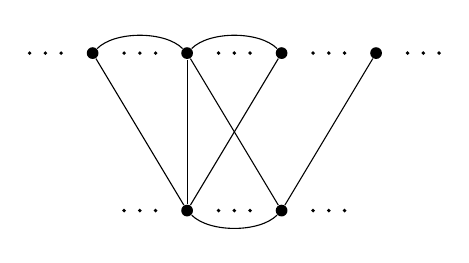
\begin{tikzpicture}
[node/.style={fill,circle,inner sep = 1.5pt},
dot/.style={fill,circle,inner sep = 0.5pt}]

\draw (-3.2,2) node[dot] {};
\draw (-3,2) node[dot] {};
\draw (-2.8,2) node[dot] {};
\draw (-2.4,2) node[node,label=90:{}] (vi1) {};
\draw (-2,2) node[dot] {};
\draw (-1.8,2) node[dot] {};
\draw (-1.6,2) node[dot] {};
\draw (-1.2,2) node[node,label=90:{}] (vi2) {};
\draw (-.8,2) node[dot] {};
\draw (-.6,2) node[dot] {};
\draw (-.4,2) node[dot] {};
\draw (0,2) node[node,label=90:{}] (vi3) {};
\draw (.4,2) node[dot] {};
\draw (.6,2) node[dot] {};
\draw (.8,2) node[dot] {};
\draw (1.2,2) node[node,label=90:{}] (vi4) {};
\draw (1.6,2) node[dot] {};
\draw (1.8,2) node[dot] {};
\draw (2,2) node[dot] {};

\draw (vi1) .. controls +(45:0.4cm) and +(135:0.4cm) .. (vi2);
\draw (vi2) .. controls +(45:0.4cm) and +(135:0.4cm) .. (vi3);

\draw (-2,0) node[dot] {};
\draw (-1.8,0) node[dot] {};
\draw (-1.6,0) node[dot] {};
\draw (-1.2,0) node[node,label=-120:{}] (uj1) {};
\draw (-0.8,0) node[dot] {};
\draw (-0.6,0) node[dot] {};
\draw (-0.4,0) node[dot] {};
\draw (0,0) node[node,label=-60:{}] (uj2) {};
\draw (0.4,0) node[dot] {};
\draw (0.6,0) node[dot] {};
\draw (0.8,0) node[dot] {};

\draw (uj1) .. controls +(-45:0.4cm) and +(-135:0.4cm) .. (uj2);

\draw (vi1) -- (uj1);
\draw (vi2) -- (uj1);
\draw (vi3) -- (uj1);
\draw (vi2) -- (uj2);
\draw (vi4) -- (uj2);
\end{tikzpicture}
\end{minipage}
\begin{minipage}[t]{0.45\linewidth}
\vspace{0pt}
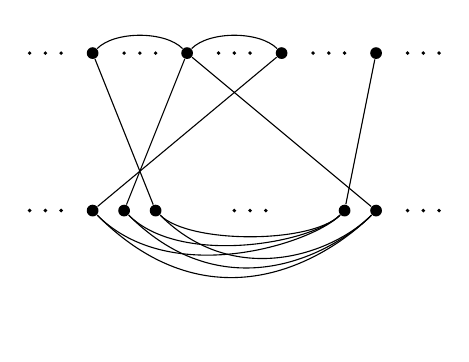
\begin{tikzpicture}
[node/.style={fill,circle,inner sep = 1.5pt},
dot/.style={fill,circle,inner sep = 0.5pt}]


\draw (-3.2,2) node[dot] {};
\draw (-3,2) node[dot] {};
\draw (-2.8,2) node[dot] {};
\draw (-2.4,2) node[node,label=90:{}] (vi1) {};
\draw (-2,2) node[dot] {};
\draw (-1.8,2) node[dot] {};
\draw (-1.6,2) node[dot] {};
\draw (-1.2,2) node[node,label=90:{}] (vi2) {};
\draw (-.8,2) node[dot] {};
\draw (-.6,2) node[dot] {};
\draw (-.4,2) node[dot] {};
\draw (0,2) node[node,label=90:{}] (vi3) {};
\draw (.4,2) node[dot] {};
\draw (.6,2) node[dot] {};
\draw (.8,2) node[dot] {};
\draw (1.2,2) node[node,label=90:{}] (vi4) {};
\draw (1.6,2) node[dot] {};
\draw (1.8,2) node[dot] {};
\draw (2,2) node[dot] {};

\draw (vi1) .. controls +(45:0.4cm) and +(135:0.4cm) .. (vi2);
\draw (vi2) .. controls +(45:0.4cm) and +(135:0.4cm) .. (vi3);

\draw (-3.2,0) node[dot] {};
\draw (-3,0) node[dot] {};
\draw (-2.8,0) node[dot] {};
\draw (-2.4,0) node[node,label=-90:{}] (uj11) {};
\draw (-2,0) node[node] (uj12) {};
\draw (-2.25,0.55) node[] {};
\draw (-1.6,0) node[node,label=5:{}] (uj13) {};
\draw (-0.6,0) node[dot] {};
\draw (-0.4,0) node[dot] {};
\draw (-0.2,0) node[dot] {};
\draw (0.8,0) node[node,label=175:{}] (uj21) {};
\draw (1.2,0) node[node,label=-75:{}] (uj22) {};
\draw (1.6,0) node[dot] {};
\draw (1.8,0) node[dot] {};
\draw (2,0) node[dot] {};



\draw (uj11) .. controls +(-45:1.4cm) and +(-135:0.6cm) .. (uj21);
\draw (uj12) .. controls +(-45:1cm) and +(-135:0.6cm) .. (uj21);
\draw (uj13) .. controls +(-45:0.6cm) and +(-135:0.6cm) .. (uj21);
\draw (uj11) .. controls +(-45:2.2cm) and +(-135:0.8cm) .. (uj22);
\draw (uj12) .. controls +(-45:1.8cm) and +(-135:0.8cm) .. (uj22);
\draw (uj13) .. controls +(-45:1.4cm) and +(-135:0.8cm) .. (uj22);

\draw (vi1) -- (uj13);
\draw (vi2) -- (uj12);
\draw (vi3) -- (uj11);
\draw (vi2) -- (uj22);
\draw (vi4) -- (uj21);
\end{tikzpicture}
\end{minipage}
\end{center} \vspace*{-1cm}
\caption{Illustration of the splitting operation when applied to vertices  and .}\vspace*{-0.5cm}
\label{fig:splitting}
\end{figure}

Let  be the graph resulting from  by splitting every vertex in  and every vertex in  (in an arbitrary order), where  is the graph resulting from splitting the vertices in  and  that resulting from splitting the vertices of . Let  be the set of edges having one endpoint in  and the other in ,  defined by  for , and let  and  be the orders on  and , respectively, resulting from  after the splitting operation.

\begin{lemma}
\label{lem:splitting}
The graph  satisfies the properties: (i) for every  we have ;\footnote{The degree of a vertex in  may be unbounded.} (ii) in the graph  every vertex has degree exactly 1 (in particular  for every ), and (iii) the instance  is a yes-instance of p-OLSE if and only if  is.
\end{lemma}

\begin{proof}
(i) Consider a vertex  that is split from vertex .  is adjacent in  to every vertex that was split from a neighbor of .  Since  has at most  many neighbors in , and since every neighbor of  was split into at most  vertices, it follows that  has at most  many neighbors in .

(ii) After splitting a vertex , all resulting vertices are of degree 1 in .  Moreover,  splitting the neighbors of  does not change the degree of  in .  Therefore, all vertices have degree 1 in  after splitting.

(iii) First, we show that if the instance  is a yes-instance of p-OLSE then  is also a yes-instance.  Let  be a subgraph of  where  and let  be a valid embedding.  Let  and  where , without loss of generality, suppose that  was split before .  After splitting  and before splitting  there is exactly one vertex  resulting from splitting  such that there is an edge between  and .  After splitting  there exists exactly one vertex  resulting from splitting  such that there is an edge .  Add  to the constructed solution  in   and define (the constructed embedding) .  Given that for any two vertices  and vertices  split from  and  (and similarly for vertices in  and ),  if and only if , and  if and only if , it follows that  is a valid embedding from  into .

Conversely, we show that if  is a yes-instance of p-OLSE then so is .  Let  be a subgraph of  where  and let  be a valid embedding.  For each pair of vertices  and  where  there are vertices  and  such that  and  were split from  and , respectively, and .  Furthermore, for each pair of vertices ,  and  are split from vertices , respectively, where .  Thus we can define a subgraph  of  where  if any vertex  split from  is in  and a map  where  if .  Given that for any two vertices  and vertices  split from  and  (and similarly for vertices in  and ),  if and only if , and  if and only if , it follows that  is a valid embedding that embeds  into .
\end{proof}

Next, we perform the following operation, denoted {\bf Simplify}, to . Observe that every vertex in  has degree 1 by part (ii) of Lemma~\ref{lem:splitting}. Let  and let  and . If either (1)  but , or (2) both  and , then we can remove edge  from  in case (1) and we can remove both edges  and  in case (2) without affecting any embedding constraint. Without loss of generality, we will still denote by  the resulting instance after the removal of the edges satisfying cases (1) and (2) above. Note that  at this point, and hence if  then no valid list embedding can be defined on a subgraph that includes both  and . Note also that  is a realization of a permutation graph  in which the vertices of  can be arranged on one line according to the order induced by , and the vertices of  can be arranged on a parallel line according to the order induced by . The vertex-set of  corresponds to the edges in , and two vertices in  are adjacent if and only if their two corresponding edges cross. Note that two vertices in  correspond to two edges of the form  and , where  and .
Let  be the graph whose vertex-set is  and whose edge set is , where  is the set of {\em conflict edges}; that is,  consists of the permutation graph  plus the set of conflict edges , where each edge in  joins two vertices in  whose corresponding endpoints in  cannot both be part of a valid solution.

\begin{lemma}
\label{lem:boundedconflictdegree}
For every vertex , the number of conflict edges incident to  in , denoted , is at most .
\end{lemma}

\begin{proof}
By part (i) of Lemma~\ref{lem:splitting}, the degree of a vertex  is at most .  Note that every conflict edge incident to  corresponds to an edge in  incident to some .  Thus for each vertex  the vertex  incident to  has at most  neighbors.  The result follows.
\end{proof}


\begin{lemma}
\label{lem:equivalence}
The instance , and hence \\ , before {\bf Simplify} is applied is a yes-instance of p-OLSE if and only if  has an independent set of size .
\end{lemma}

\begin{proof}
A size- independent set  in  corresponds to a set of  edges  in  such that ,
, and  is a subgraph in  whose vertices form an independent set. Clearly, the embedding , , is a valid embedding that embeds  into  because it respects both , and because it respects the embedding constraints. To see why the latter statement is true, note that, for any two vertices  and  () in , either there was no edge between  and  before the application of the operation {\bf Simplify}, or there was an edge and got removed by {\bf Simplify}, and in this case there must be also an edge between  and  in ; in either case,  respects the embedding constraints.

Conversely, let  be a valid embedding that embeds a subgraph  of size  where , and , for . We claim that the set of vertices  is an independent set in . Since  is a valid list embedding, no edge in  exists between any two vertices in . Let  and  be two vertices in , where . If there is no edge between  and  in , then no edge exists between  and  in . On the other hand, if there is an edge between  and  in , then because  is a valid embedding, there must be an edge as well between  and . After applying {\bf Simplify}, the edge between  and  will be removed, and hence no edge exists between  and  in . It follows that  is a size- independent set in .\end{proof}

\begin{lemma}\label{lem:separation}
Let  be a hereditary class\footnote{The class  is closed under taking subgraphs; that is, every subgraph of a graph in  is also in .} of graphs on which the {\sc Independent Set} problem is solvable in polynomial time, and let  be a fixed integer constant. Let , where at most  edges in   are incident to any vertex in .  Assuming that a graph in  is given as  ( is given), the {\sc Independent Set} problem can be solved in  time on graphs in the class .
\end{lemma}

\begin{proof}
Let  be an instance of {\sc Independent Set}, where .
We use the random separation method introduced by Cai et al.~\cite{cai}; this method can be de-randomized in fpt-time using the notion of universal sets and perfect hash functions~\cite{alon95,naor,schmidt}.

We apply the random separation method to the subgraph , and color the vertices in  with two colors, ``green" or ``red", randomly and independently. If  is an independent set of size  in , since there are at most  edges of  that are incident to any vertex in , the probability that all vertices in  are colored green and all their neighbors along the edges in  are colored red, is at least . If a size- independent set exists, using universal sets and perfect hash functions, we can find a 2-coloring that will result in the independent set vertices being colored green, and all their neighbors along edges in  being colored red in time . Therefore, it suffices to determine, given a 2-colored graph , whether there is an independent set of size  consisting of green vertices whose neighbors along the edges in  are red vertices. We explain how to do so next.


Suppose that the vertices in  are colored green or red, and let  be the subgraph of  induced by the green vertices, and  that induced by the red vertices. Notice that if there is an independent set  consisting of  green vertices whose neighbors along the edges in  are red, then for each vertex  in ,  is an isolated vertex in the graph . Moreover, since  is an independent set, then no edge in  exists between any two vertices in . Therefore, if we form the subgraph , where  is the set of vertices in  that are isolated with respect to the set of edges , and  is the set of edges in  whose both endpoints are in , then  is an independent set in . On the other hand, any independent set of  is also an independent set of .  Since  is a subgraph of  and  is hereditary, it follows that  and we can compute a maximum independent set  in  in polynomial time. If , then we accept the instance; otherwise, we try the next 2-coloring. If no 2-coloring results in an independent set of size at least , we reject. From the above, given a 2-coloring, clearly we can decide if there is an independent set of size  consisting of green vertices whose neighbors along the edges in  are red vertices. The result follows.\end{proof}


\begin{theorem}
\label{thm:mainboundeddegree}
The p-OLSE problem restricted to instances in which  and  is .
\end{theorem}

\begin{proof}
Let  be an instance of p-OLSE in which both  and  are upper bounded by a fixed constant. We form the graph  and perform the splitting operation described in Definition~\ref{def:splitting} to obtain the instance . By Lemma~\ref{lem:splitting},  is a yes-instance of p-OLSE if and only if  is. We apply the operation {\bf Simplify} to the instance and construct the graph  as described above, where  is a permutation graphs. Note that the set of edges  is known to us. By Lemma~\ref{lem:equivalence},  is a yes-instance of p-OLSE if and only if  has an independent set of size . Observe that we can perform the splitting and the {\bf Simplify} operations, and construct  in polynomial time. Since the {\sc Independent Set} problem is solvable in polynomial time on the class of permutation graphs (\eg, see~\cite{kim}), the class of permutation graphs is hereditary, and every vertex in  has at most  edges in  incident to it by Lemma~\ref{lem:boundedconflictdegree}, it follows from Lemma~\ref{lem:separation} that we can decide if  has an independent set of size  in fpt-time, and hence decide the instance  in fpt-time. \end{proof}

Unfortunately, the above result does not hold true for p-OLISE, even when , , and , because the number of vertices in  that have the same vertex  in their list may be unbounded.

From Proposition~\ref{prop:whardness}, we know that in the case when  is unbounded, and both  and , p-OLSE is -hard. The following proposition says that the condition  is essential for this -hardness result:

\begin{proposition}
\label{prop:randomsimple}
The p-OLSE and p-OLISE problems restricted to instances in which ,  (resp.  and  for p-OLISE by symmetry) and  are .
\end{proposition}

\begin{proof}
We prove the result for p-OLSE. The proof is exactly the same for p-OLISE. The proof uses the random separation method, but is simpler than the proof of Lemma~\ref{lem:separation}. Let  be an instance of p-OLSE. Observe that if  is the solution that we are looking for then  must be an independent set since . Use the random separation method to color  with green or red. Since , if a solution  exists, then in fpt-time (deterministic) we can find a 2-coloring in which all vertices in  are green and their neighbors in  are red. So we can work under this assumption. Let  be the subgraph of  induced by the green vertices, and  that induced by the red vertices. Observe that any green vertex in  that is not isolated in  can be discarded by our assumption (since all neighbors of a vertex in  must be in ). Therefore, we can assume that  is an independent set. We can now compute a maximum cardinality subgraph of  that can be (validly) embedded into  using the dynamic programming algorithm in Proposition~\ref{prop:noedges}; if the subgraph has size at least  we accept; otherwise, we try another 2-coloring of . If no 2-coloring of  results in a solution of size at least , we reject.\end{proof}



\section{Parameterization by the Vertex Cover Number}
\label{sec:vcnumber}
In this section we study the parameterized complexity of p-OLSE parameterized by the size of a vertex cover  in the graph , shortly (p-VC-OLSE), defined formally as follows:

\paramproblem{} {Two graphs  and  with linear orders  and  defined on the vertices of  and ; a function ; and }{ where  is the size of a minimum Vertex Cover}{Is there a subgraph  of  of  vertices and an injective map  such that: (1)  for every ; (2) for every , if  then ; and (3) for every ,  if and only if } \\

As noted earlier, the reduction used in Proposition~\ref{prop:whardness} to prove the -hardness of p-OLSE when restricted to instances in which ,  and  results in an instance in which the number of vertices in , and hence , is upper bounded by a function of the parameter. Since  it follows immediately that p-VC-OLSE is -hard in this case.  Therefore:

\begin{proposition}
\label{prop:whardnessvc}
p-VC-OLSE restricted to instances in which  and  is -complete.
\end{proposition}

\vspace*{-1mm}
Therefore, we can focus our attention on studying the complexity of p-VC-OLSE restricted to instances in which .
\vspace*{-1mm}
\begin{theorem}
\label{thm:fptvslose}
p-VC-OLSE restricted to instances in which  can be solved in time  and hence is .
\end{theorem}
\vspace*{-3mm}
\begin{proof}
Let  be any fixed integer, and suppose that . Let  be an instance of p-VC-OLSE, where  is the desired solution size and  is the size of a vertex cover in . In fpt-time (in  time~\cite{ckxvc}) we can compute a vertex cover  of  of size  (if no such vertex cover exists we reject the instance). Let , and note that  is an independent set of . Suppose that the solution we are seeking (if it exists) is , and the valid mapping of  is . Let , where  is possibly empty, and let  be the restriction of  to . We enumerate each subset of  as  in time , enumerate each possible mapping from  to  as  in time , and check the validity of  in polynomial time (if no valid  exists, we reject the enumeration); since , the enumeration can be carried out in time . Therefore, we will work under the assumption that the desired solution intersects  at a known subset , and that the restriction of  to  is a known map , and reject the instance if this assumption is proved to be wrong.

We remove all vertices in  from  (together with their incident edges) and update  accordingly; without loss of generality, we will still use  to refer to the resulting graph whose vertex-set at this point is . Let  be the vertices in , where . Since  is valid, we have . We now perform the following operation. For each vertex  in  and each vertex , if setting  violates the embedding constraint in the sense that either (1) there is a vertex  such that  but  or (2) there is a vertex  such that  (resp. ) but  (resp. )), then remove  from . Afterwards, partition the vertices in  into at most  intervals, , where  consists of the vertices preceding  (with respect to ),  consists of those vertices following , and  consists of those vertices that fall strictly between vertices  and , for . Similarly, partition  into  intervals, , where  consists of the vertices preceding  (with respect to ),  those vertices following , and  those vertices that fall strictly between vertices  and , for . Clearly, any valid mapping  that respects  and  must map vertices in the solution that belong to  to vertices in , for , in a way that respects the restrictions of  and  on  and , respectively. On the other hand, since after the above operation every vertex  in  can be validly mapped to any vertex , any injective mapping  that maps a subset of vertices in  to a subset in  in a way that respects the restrictions of  and  to  and , respectively, can be extended to a valid embedding whose restriction to  is . Therefore, our problem reduces to determining whether there exist injective maps , , mapping vertices in  to vertices in , such that the total number of vertices mapped in the 's is . Consider the subgraphs  and , for . Since  is an independent set, the presence of edges in  does not affect the existence of a valid list mapping from vertices in  to , and hence those edges can be removed. Therefore, we can solve the opt-OLSE problem using Proposition~\ref{prop:noedges} on the two graphs  and  to compute a maximum cardinality subset of vertices  in  that can be validly embedded into  via an embedding . If the union of the 's with  has cardinality at least , we accept. If after all enumerations of  and  we do not accept, we reject the instance. This algorithm runs in time . \end{proof}

\section{Conclusion}\label{sec:conclusion}
We drew a complete complexity landscape of p-OLSE and p-OLISE, and their optimization versions, with respect to the computational frameworks of classical complexity, parameterized complexity, and approximation, in terms of the structural parameters ,  and .  We also showed that relaxing the order constraint of p-OLSE and p-OLISE makes the problems significantly easier (in ).
There are few interesting open questions that result from our research:


\begin{enumerate}
  \item  What is the complexity of the weighted versions of the problems presented in this paper (vertex-weights or edge-weights), with respect to the frameworks of classical complexity, approximation, and parameterized complexity?
   \item Are there meta-theorems, possibly similar to those for the {\sc Subgraph Isomorphism} and {\sc Graph Embedding} problems (see~\cite{grohebook}), in terms of the structures of  and/or , that would unify some of the complexity results about p-OLSE and p-OLISE presented in the paper?

   \item Finally, graph representations of proteins in practice often fall within the bounds of the parameters assumed for the fixed-parameter algorithms (and approximation algorithms) presented in the paper. How do these algorithms perform in practice?

  \end{enumerate}

\bibliographystyle{plain}
\bibliography{paper}



\end{document}
